\documentclass{article}
\usepackage[utf8]{inputenc}

\usepackage{amsfonts}
\usepackage{amsmath}

\usepackage{float}
\usepackage{graphicx}
\usepackage{subcaption}
\usepackage{caption}

\author{Kody Manastyrski}
\date{October, 2021}
\title{CP 8318 Assignemnt 2}


\begin{document}

\maketitle

\section{}
\subsection{Question 3}
The resulting line for logistic regression gives the appearance of a more true
division between the two groups.
On the other hand the GDA line lands where would likely be the actual middle of
the two, which implies that that is the overlap of the two distributions.
From this it seems that logistic regression will fit well for a specific dataset
(in this scenario), while the GDA will fit better for the `general' case. 
By this, I mean that as we see more data, the logistic regression will create a
more accurate division while the GDA will remain unchanged since it is working 
from the underlying distribution.

\begin{figure}[h]
	\centering
	\begin{subfigure}{.49\textwidth}
		\centering
		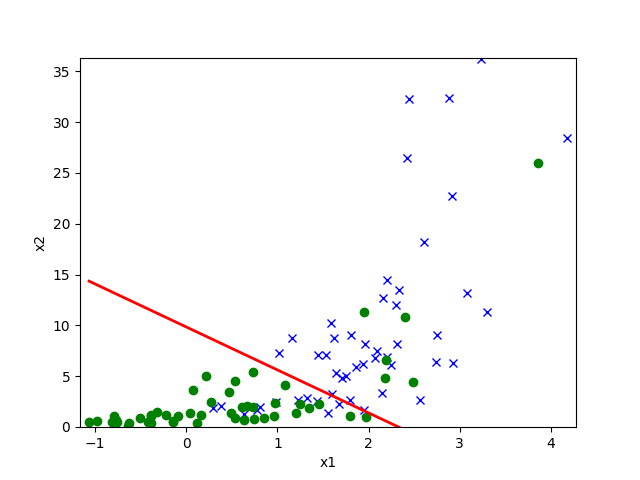
\includegraphics[width=\textwidth]{src/linearclass/ds1/logreg_pred_1.txt.png}
		\caption{Log Reg}
		\label{fig:set one LR}
	\end{subfigure}
	\hfill
	\begin{subfigure}{.49\textwidth}
		\centering
		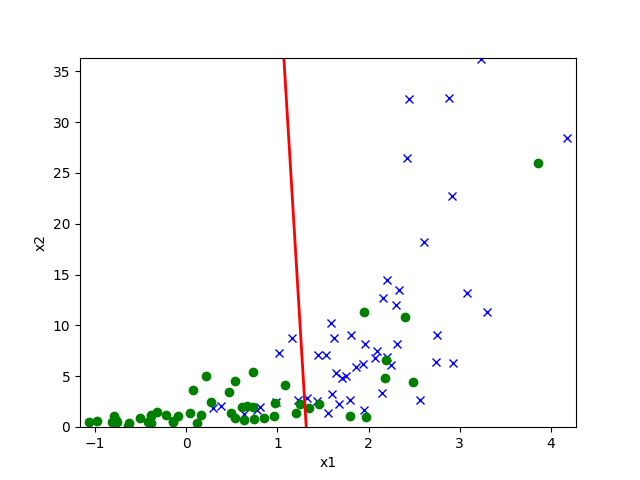
\includegraphics[width=\textwidth]{src/linearclass/ds1/gda_pred_1.txt.png}
		\caption{GDA}
		\label{fig:set one GDA}
	\end{subfigure}
\end{figure}


\subsection{Question 4}

In this case, the two seem quite similar. 
The difference is only visible (in the given figures) at the x-intercept, and 
even then zooming in is required. 
The logistic regression is further from an intercept of 4 than the GDA is, but
only slightly. 
Checking the count of datapoints in the files we have 800 in the training files,
and 100 in the valid files. 
This is the same for the previous example, and thus the only conclusion here is
that the logistic regression was quite close by coincidence. 
Indeed, with this dataset there appears to be a more identical form to the
two distributions. 
Perhaps its this apparent fact that leads to the result that we have here.

\begin{figure}[h]
	\centering
	\begin{subfigure}{.49\textwidth}
		\centering
		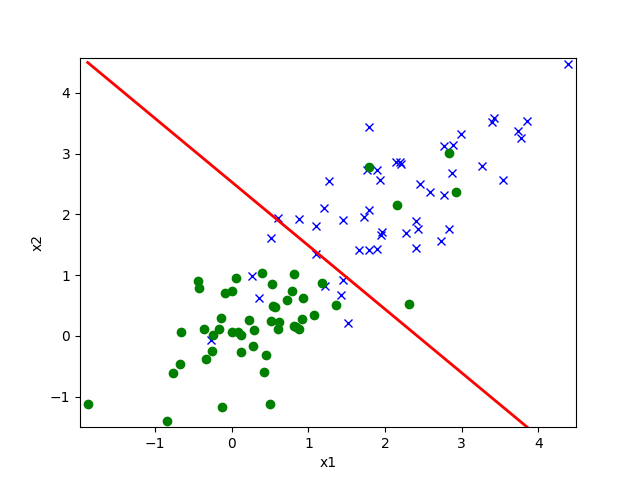
\includegraphics[width=\textwidth]{src/linearclass/ds2/logreg_pred_2.txt.png}
		\caption{Log Reg}
		\label{fig:set two LR}
	\end{subfigure}
	\hfill
	\begin{subfigure}{.49\textwidth}
		\centering
		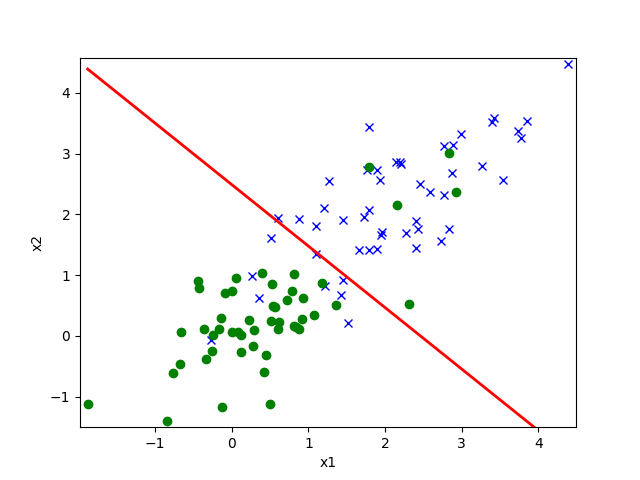
\includegraphics[width=\textwidth]{src/linearclass/ds2/gda_pred_2.txt.png}
		\caption{GDA}
		\label{fig:set two GDA}
	\end{subfigure}
\end{figure}

\subsection{Question 5}

I suspect that normalizing the distributions, and then translating them so that 
only their tails overlap would potentially affect the results in the first 
dataset. 
It appears that the first dataset has a platykurtic (group a) distribution and
a leptokurtic (group b) distribution which seems to be skewed toward the left.
This being the case, then normalizing them and translating the two so that 
quartile 4 of group a overlaps with quartile 1 of group b may yield significantly
better results since that seems to be the ideal situation for GDA (supposing the
data point count is not too high).

\section{}
\subsection{Question 1}
\begin{center}
	\begin{align*}
		p(y; \lambda) &= \frac{e^{-\lambda}\lambda^y}{y!} \\
					  &= e^{
					  ln(
				  \frac{
			  e^{-\lambda}\lambda^y}{y!}
		  )} \\
		  &=  e ^{
			  ln(
			  e^{-\lambda}
			  )
			  + ln(\lambda^y)
			  - ln(y!)
		  } \\
			&= e^{ln(
				  -\lambda + yln(\lambda) - ln(y!))
			  }\\
			&= e^{
				ln(-\lambda + yln(\lambda))
			} e^{-ln(y!)}\\
			&= \frac{1}{y!}e^{yln(\lambda) - \lambda}
	\end{align*}
\end{center}
Thus we have natural parameters:
\[ b(y) = \frac{1}{y!} \]
\[ \eta = ln(\lambda) \]
\[ T(y) = y \]
\[ a(\eta) = \lambda \]

\subsection{Question 2}
\begin{center}
	\begin{align*}
		g(n) &= E\left[ y; \eta \right ]\\
			 &= E\left[ p(y; \eta) \right] \\
			 &= E\left[ b(y)e^{\eta^TT(y)-a(n)} \right]\\
			 &= \frac{d}{d \eta}\left( \frac{e^{ln(\lambda)^Ty - \lambda}}{y!}\right )\\
			 &= \frac{d}{dy}\frac{d}{ln(\lambda)}\left( \frac{e^{ln(\lambda)^Ty-\lambda}}{y!}\right )\\
			 &= \frac{\frac{d}{dy}\frac{d}{d \lambda}ln(\lambda)^ty -\lambda e^{ln(\lambda)^Ty-\lambda}}
			 {\frac{d}{dy} \frac{d}{d ln(\lambda)}y! }\\
			 &= \frac{d}{dy}\frac{d}{dln(\lambda)}
	 \end{align*}
\end{center}
\subsection{}

\end{document}


